\subsection{On confidence intervals}

Figure \ref{fig:ci} shows the impact of our diversion policy
for the 3 site case with a 60 minute lead time, by examining the
change of performance instead of simply the performance.
The confidence intervals show that the performance improvement
from our diversion policy is statistically
significant. Also, note that as we increase the fraction of
volunteers, the variance also increases. The reason is that,
when there are more volunteers, there are more diversions which
induce greater variance. If we examine the performance improvement
for other metrics or for other levels of granularity, similar patterns
can be observed.

\begin{figure}[htp]
\centering
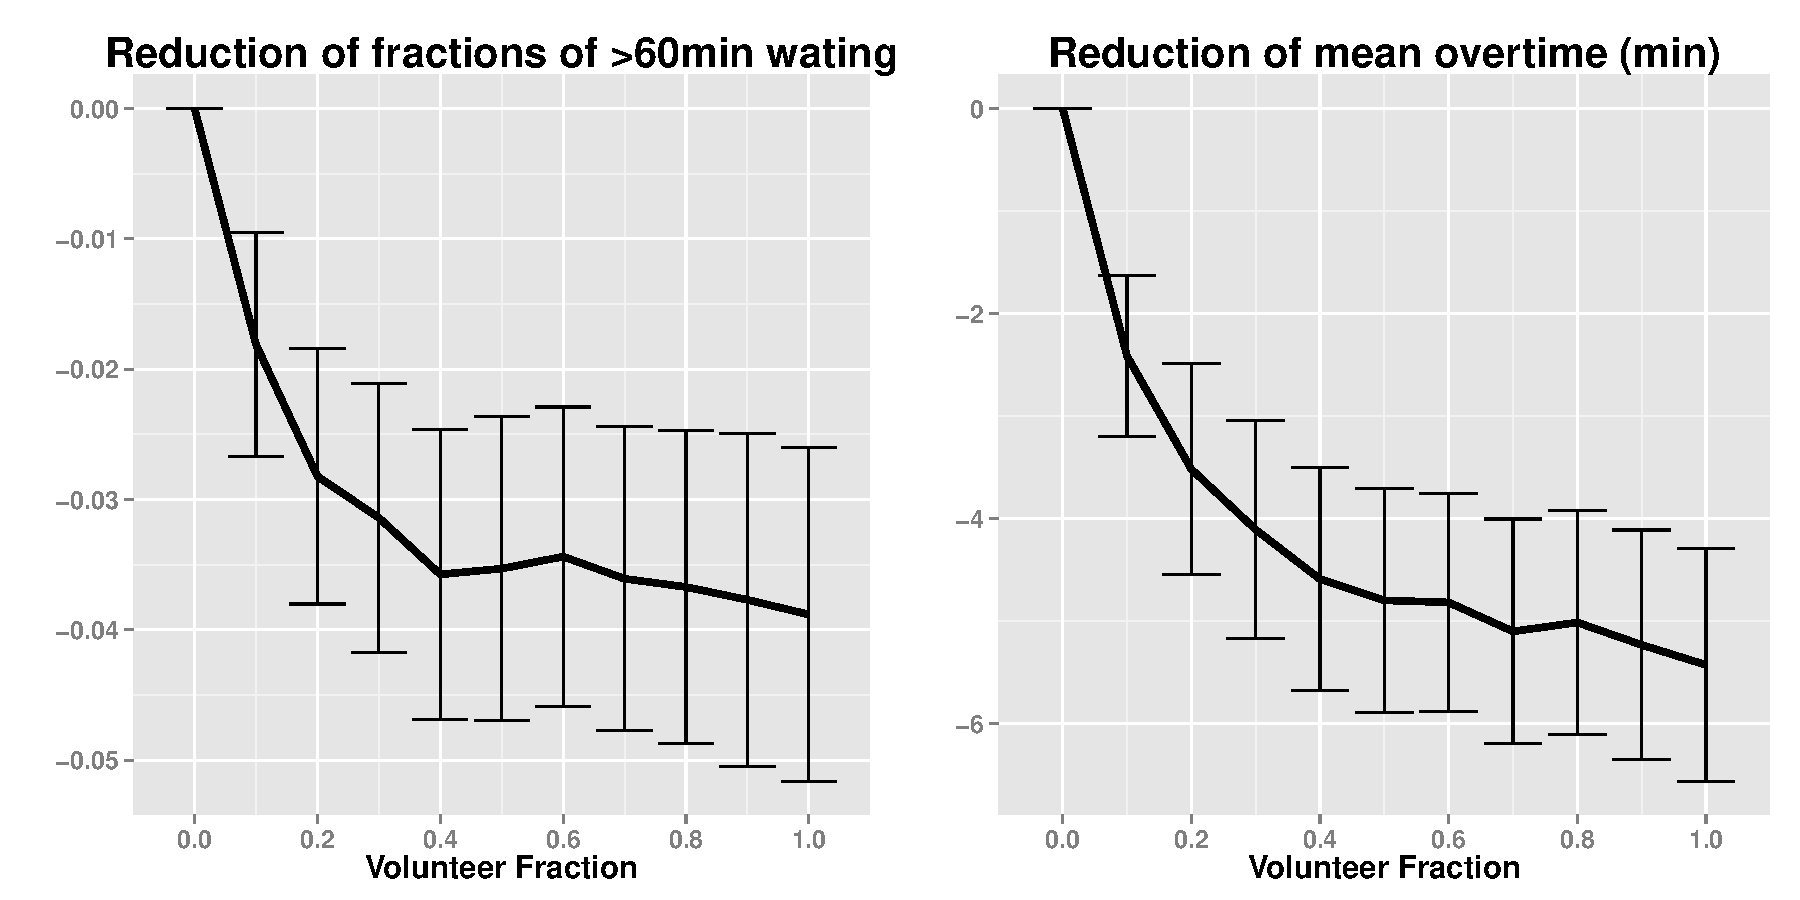
\includegraphics[width=.95\textwidth]{chap3/numeric/pic/ci}
\caption{The impact of diversion policy for the 3 site case
with a 60 minute lead time. The left plot is showing the
reduction of fractions of over 60 minute waiting. The right plot
is showing the reduction of mean overtime.}
\label{fig:ci}
\end{figure}
